\subsection{Berechnung der Suszeptibilität}
Die magnetische Flussdichte $\vec{B}$ ergiebt sich aus der magnetischen Feldstärke $\vec{H}$ und der Induktionskonstante $\mu_0$.
Zusetzlich wird bei Anwesenheit einer Materie die Magnetisierung M addiert.
\begin{align*}
  \vec{B}=\mu_0 \vec{H}+M
\end{align*}
M setzt sich aus dem mittleren magnetischen Moment $ \overline{\vec{\mu}}$ und der Zahl N der Momete pro Volumeneinheit zusammen.
\begin{align*}
  \vec{M}=N\mu_0\overline{\vec{\mu}}
\end{align*}
Die Magnetisierung $\vec{M}$ kann auch ausgedrückt werden als:
\begin{align*}
  \vec{M}=\mu_0\chi\vec{H}
\end{align*}
$\chi$ ist dabei die Suszeptibilität welche wiederum von H und der Temperatur T abhängt.
Um einen Paramagnetismus zu beobachten benötigt man Materialien die einen nicht verschwindenden Drehimpuls besitzen.
Durch die Orientierung der magnetischen Momente, welche mit den Drehimpuls gekoppelt sind, relativ zu einem äuseren Feld entsteht der Paramagnetismus.
Der Gesamtdrehimpuls $\vec{J}$ eines Atoms besteht aus drei Komponenten. Dem Bahndrehimpuls der Elektronenhülle $\vec{L}$, dem Eigendrehimpuls (Spin) der Elektronen $\vec{S}$ und dem Kerndrehimpuls. Der Kerndrehimpuls spiel beim Paramagnetismus kene große Rolle und kann daher vernachlässigt werden.
Bei kleinen Magnetfeldern gilt die LS-Kopplung.
\begin{align*}
  \vec{J}=\vec{L}+\vec{S}
\end{align*}
Aus der Quantenmechanik folgt, dass
\begin{align*}
  \vec{\mu_L}=-\frac{\mu_B}{\hbar}\vec{L}
\end{align*}
und
\begin{align*}
  \vec{\mu_S}=-g_S\frac{\mu_B}{\hbar}\vec{S}
\end{align*}
gilt. gs ist das gyromagnetische Verhältnis. Das Borsche Magneton $\mu_B$ ist dabei gegeben als
\begin{align*}
  \mu_B:=\frac{1}{2}\frac{e_0}{m_0}\hbar.
\end{align*}
Der Betrag des Gesamtdrehimpulses ist gegeben durch
\begin{align*}
  \bigl|\vec{J}\bigr|=\sqrt{J(J+1)}\hbar
\end{align*}
Somit ergiebt sich:
\begin{align*}
  \bigl|\vec{\mu_L}\bigr|=\mu_B\sqrt{L(L+1)}
\end{align*}
und
\begin{align*}
    \bigl|\vec{\mu_S}\bigr|=g_S\mu_B\sqrt{S(S+1)}.
\end{align*}

\begin{figure}[h!]
  \centering
  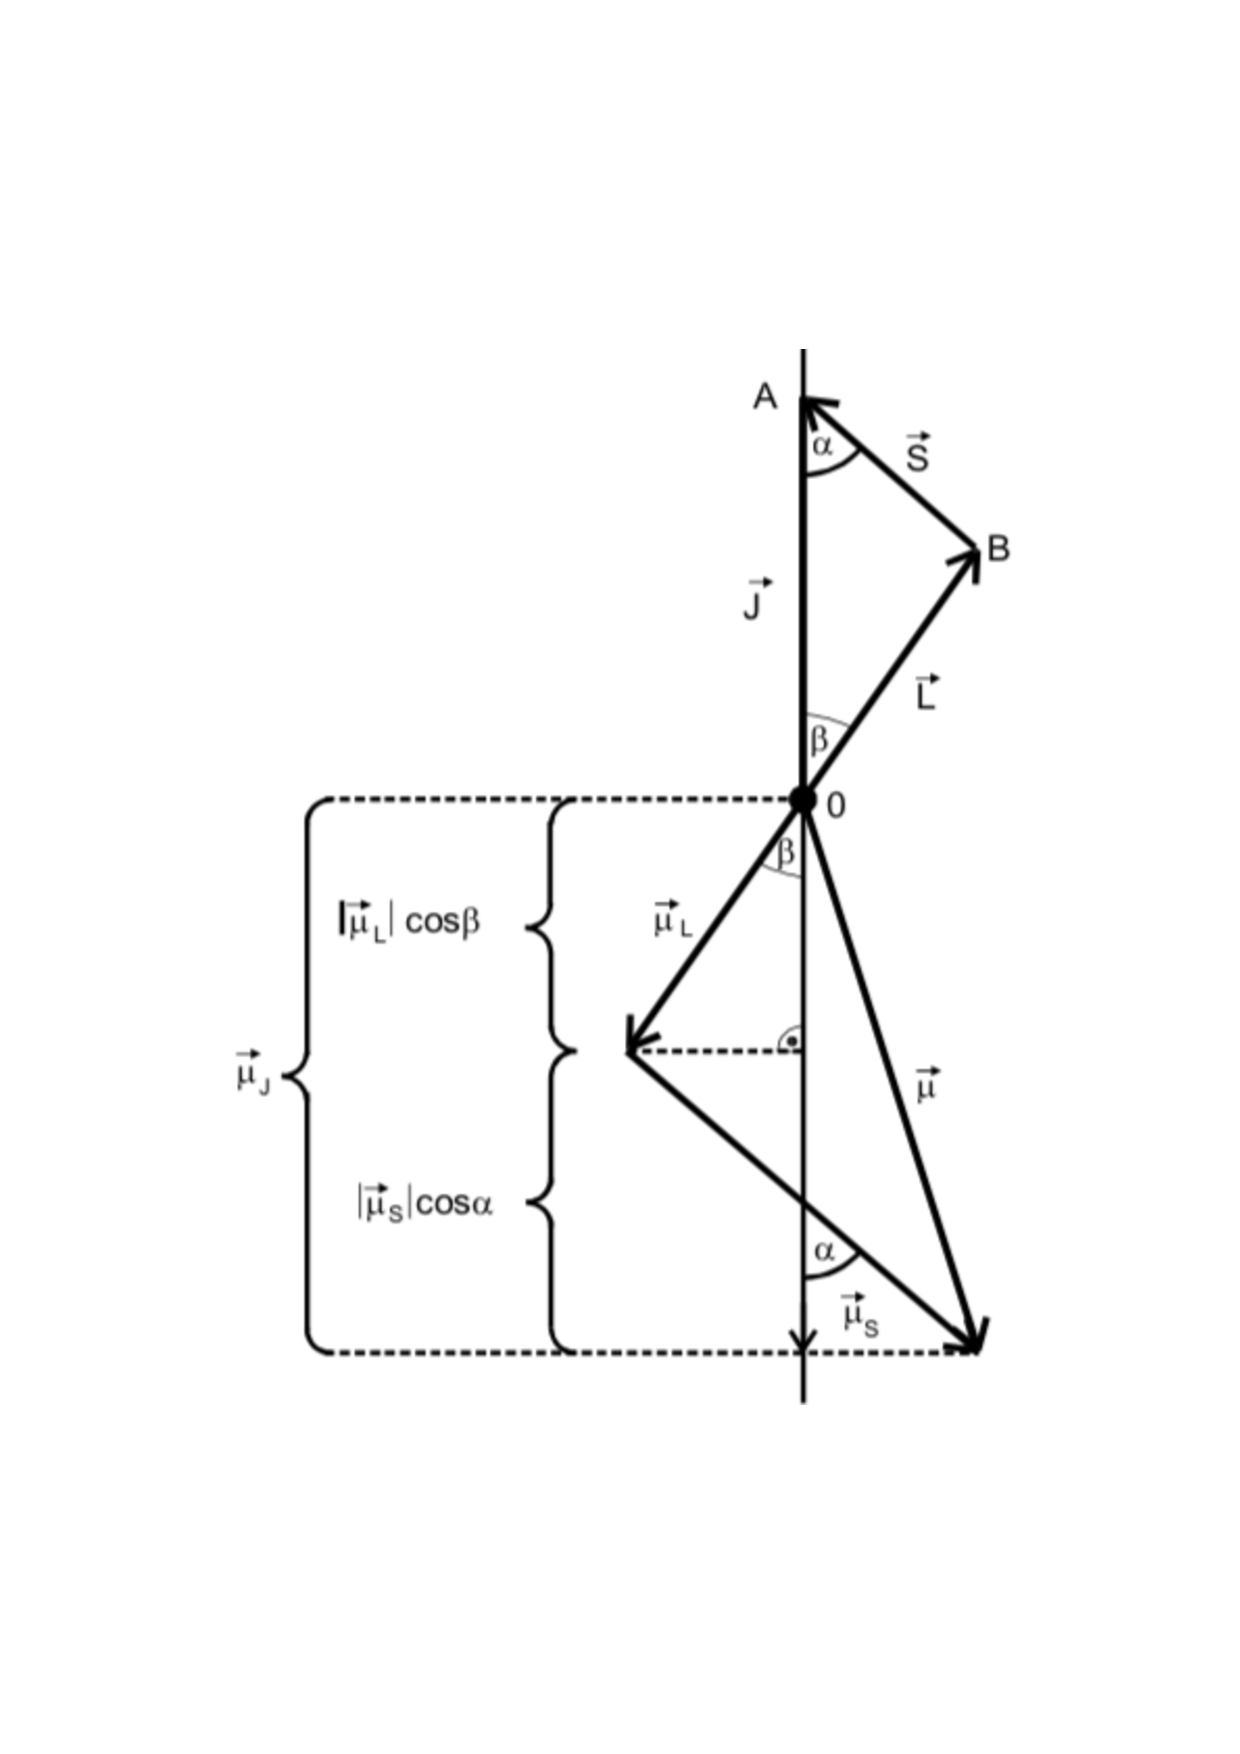
\includegraphics[width=0.8\textwidth]{606kopplung.pdf}
  \caption{Vektordiagramm aus den Drehimpulsvektoren einer Elektronenhülle und den daraus resulteirenden magnetischen Momenten \cite{1}}
  \label{fig:mMoment}
\end{figure}
Aus der Abbildung \ref{fig:mMoment} ergiebt sich nun die Beziehung
\begin{align*}
  \bigl|\vec{\mu_J}\bigr|=\bigl|\vec{\mu_S}\bigl|\text{cos}(\alpha)+\bigl|\vec{\mu_L}\bigr|\text{cos}(\beta)
\end{align*}
Mit der aus der Quantenmachanik kommenden Annahme, dass $g_S$ den Wert 2 besitzt ergiebt sich für $\bigl|\vec{\mu_B}\bigl|$ folgender Ausdruck
\begin{align*}
  \bigl|\vec{\mu_S}\bigr|=\bigl|\mu_B\bigr|\sqrt{J(J+1)}\cdot g_J
\end{align*}
$g_J$ ist der Landé-Faktor und ist gegeben durch:
\begin{align}
  g_J=\frac{3J(J+1)+S(S+1)-L(L+1)}{2J(J+1)}
  \label{eqn:lande}
\end{align}
Die aus der Quantenmechanik kommende Richtungsquantelung besagt, dass nur bestimmt Winkel zwischen $\vec{\mu_J}$ und dem äußeren Magnetfeld möglich sind.
\begin{align}
  \mu_{J_z}=-\mu_Bg_J\text{m}
  \label{eqn:mu}
\end{align}
m ist die Orientierungsquantenzahl und tritt nur ganzzahlig auf.
Der Winkel kann nur $2J+1$ verscheidene Einstellungen haben.
Jeder dieser Winkel besitzt eine bestimmte potentielle Energie mit dieser kann die Magnetisierung $\vec{M}$ berechnet werden.
Dafür wird die Häufigkeit der auftretenden Orientierungen Bestimmt. Die Wahrscheinlichkeit wird mit dem manetischen Moment aus Formel \ref{eqn:mu} multipliziert und anschleißend über alle möglichen Winkeleinstellungen summiert.
Es ergiebt sich nach Umformungen die Suszeptibilität als:
\begin{align}
  \chi=\frac{\mu_0\mu^2_Bg^2_JNJ(J+1)}{3kT}.
  \label{eqn:suszT}
\end{align}
N beschreibt die Anzahl der Momente pro Volumeneinheit. Die Boltzmannkonstante wir mit k angegeben und die Temperatur mit T.
Für hohe Temperaturen kann
\begin{align*}
  \chi\sim\frac{1}{T}
\end{align*}
angenommen werden. Diese Proportionalität ist als Curiesches Gesetz des Paramagnetismus bekannt.
Es ist bekannt, dass sich der Paramagnetismus besonders gut bei Seltenen Erden beobachten läst.
Die Elektronen in der 4f-Schale sind dafür verantwortlich. Durch die Hundschen Regeln werde die Verteilung der Elektronen innerhalb einer Schale und der daraus resultierende Gesamtdrehimpuls beschreiben.
\begin{itemize}
  \item Die Spins $\vec{s_i}$ summieren sich zu einem maximalen Gesamtspin $\vec{S}=\sum\vec{s_i}$ der nach dem Pauli-Prinzip möglich ist.
  \item Der Bahndrehimpuls $\vec{l_i}$ wir ebenfalls summiert zu $\vec{L}=\sum\vec{l_i}$. $\vec{L}$ muss mit den Pauli-Prinzip und der ersten Regel Verträglich sein.
  \item Der Gesamtdrehimpule $\vec{J}$ selzt sich, für eine mehr als halb volle Schale, zusammen aus $\vec{J}=\vec{L}+\vec{S}$. Ist die Schale hingegen weniger als halb besetzt ergiebt sich $\vec{J}=\vec{L}-\vec{S}$.
\end{itemize}

\subsection{Messung der Suszeptibilität}
\begin{figure}[h!]
  \centering
  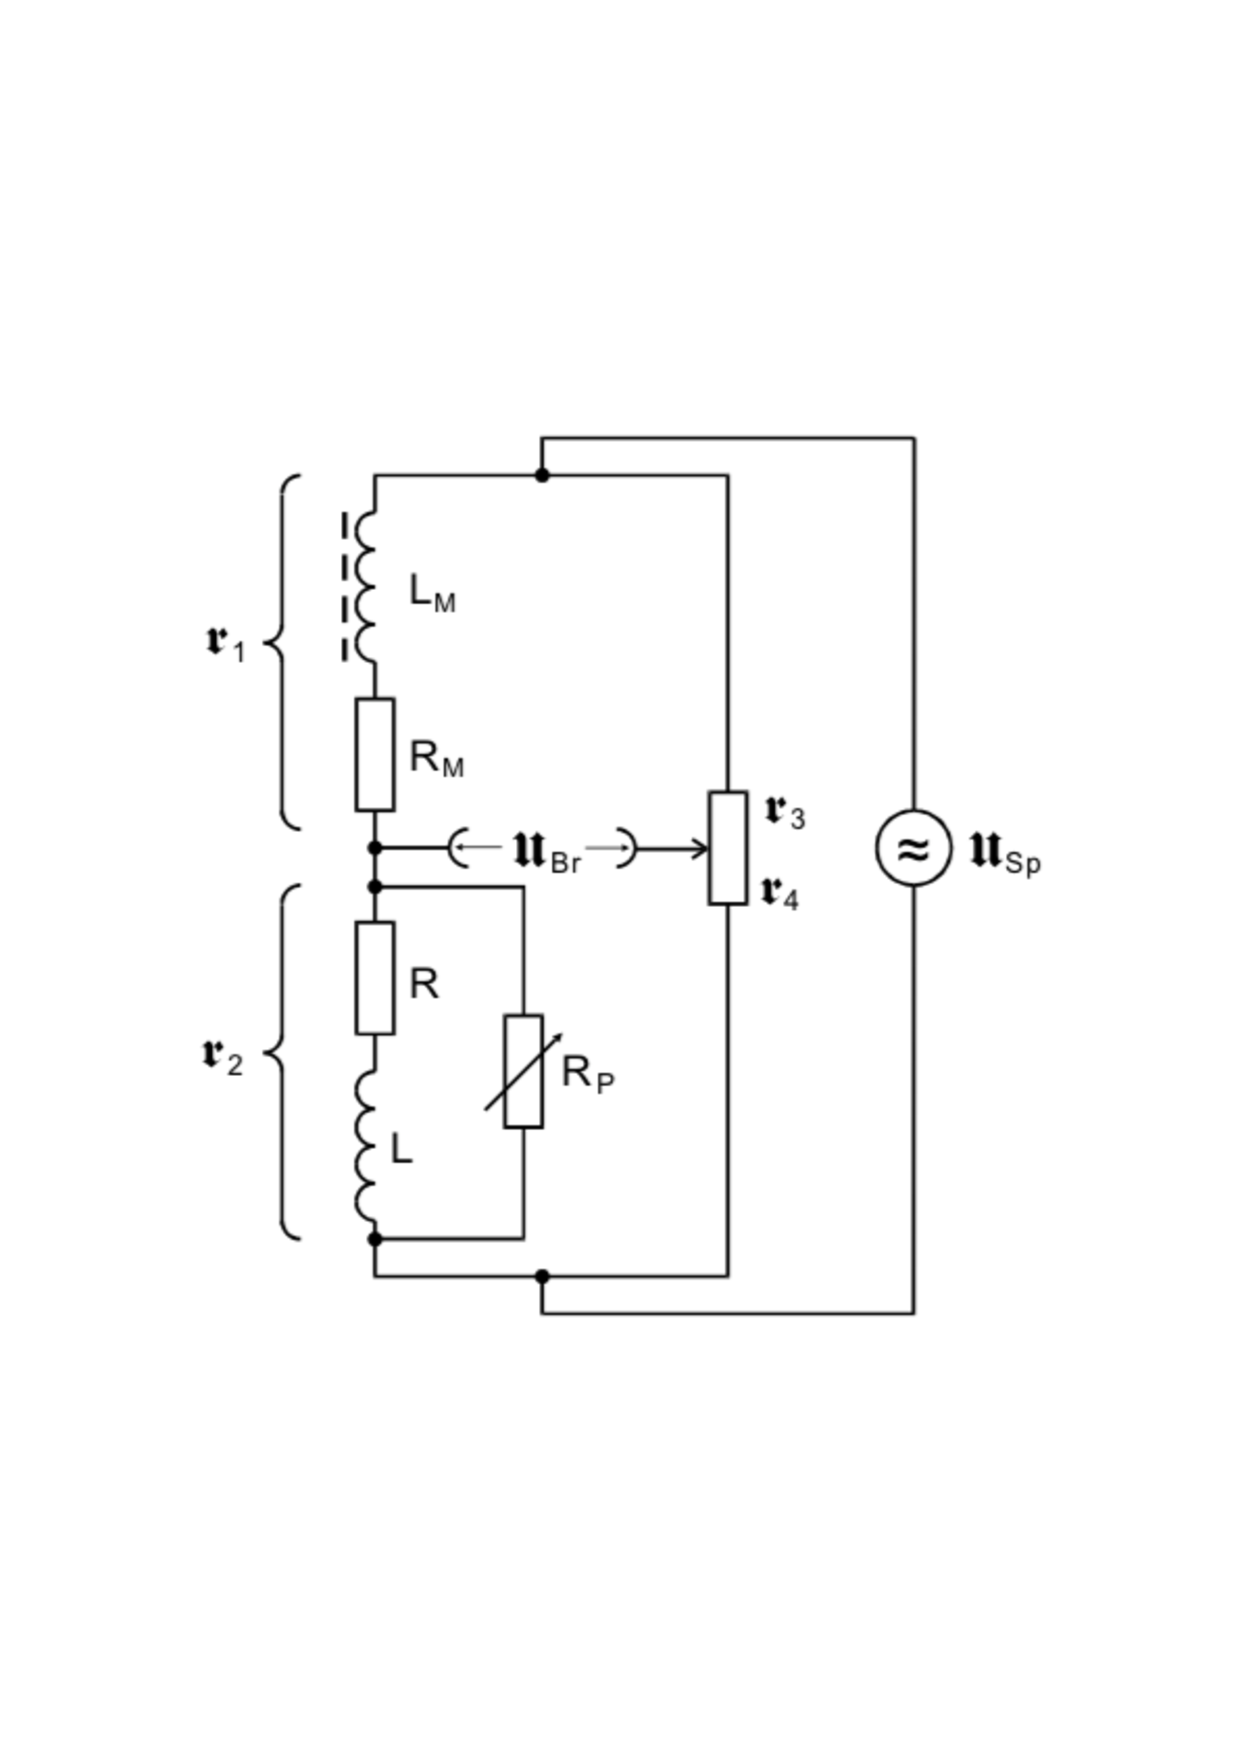
\includegraphics[width=0.8\textwidth]{606schaltung.pdf}
  \caption{Brückenschaltung für eine Suszeptibilitätsmessung \cite{1}}
  \label{fig:schalt}
\end{figure}
Die Messung der Suszeptibilität wird nun mit der in Abbildung \ref{fig:schalt} zusehenen Brückenschaltung durchgeführt.
Für die Brückenschaltung benötigt man zwei gleiche Spulen mit identischer Induktivität. Um $\chi$ zu bestimmen wird Materie in eine Spule eingeführt und die Induktivitätsdifferenz $\Delta L$ zu luftgefüllte Spule gemessen.
Die Schaltung bietet zwei Möglichkeiten die Suszeptibilität zu messen.
Zu beginn wird die Brücke angeglichen, das heißt, dass keine Brückenspannung $U_{Br}$ zu messen ist.
Füllt man nun eine Spule, mit der zu untersuchenden Materie, kann man aus der anliegenden Brückenspannung die Suszeptibilität bestimmen.
Für hohe Messfrequenzen ($\omega^2L^2>>R^2$) ergiegbt sich durch Umformungen
\begin{align}
  \chi(\omega\to\infty)=4\frac{F}{Q}\frac{U_{\text{Br}}}{U_{\text{Sp}}}.
  \label{eqn:suszU}
\end{align}
Der Spulenquerschnitt ist als F gegeben. Q bescheribt den Querschnitt der Probe und $U_{\text{Sp}}$ steht für die Speisespannung.\\
Bei der zweiten möglichen Berechnung wird nach dem Abgleichen der Brücke die Spule mit der Probe gefüllt und die Brücke erneut abgeglichen.
Mit der auftretenden Differenz der Einstellungen der Abgleichelemente läst sich über die Formel
\begin{align}
  \chi=2\frac{\Delta R}{R_3}\frac{F}{Q}
  \label{eqn:suszR}
\end{align}
ebenfalls die Suszeptibilität bestimmen. $R_3$ ist dabe der Widerstand am Potentiometer, und $\Delta R$ beschreibt die Differenz der Einstellungen.
